\documentclass[useAMS,usenatbib]{mn2e}

\voffset=-0.8in

% Packages:
\usepackage{graphicx}
\usepackage{amsmath}
\usepackage{xspace}
%\usepackage{dsfont}
\usepackage[utf8]{inputenc}
\usepackage{caption}
\usepackage{subcaption} % subfigures
\usepackage{float}

\usepackage{epstopdf} 

\title[]
{Trans-Dimensional Bayesian Inference for Gravitational Lens Substructures}
    
\author[Brewer, Huijser and Lewis]{%
  Brendon~J.~Brewer$^{1}$\thanks{To whom correspondence should be addressed. Email: {\tt bj.brewer@auckland.ac.nz}},
  David Huijser$^{1}$,
  Geraint F. Lewis$^2$
  \medskip\\
  $^1$Department of Statistics, The University of Auckland, Private Bag 92019, Auckland 1142, New Zealand\\
  $^2$Sydney Institute for Astronomy, School of Physics, A28,
  The University of Sydney, NSW 2006, Australia}

%%%%%%%%%%%%%%%%%%%%%%%%%%%%%%%%%%%%%%%%%%%%%%%%%%%%%%%%%%%%%%%%%%%%%%%%%%%%%%

\begin{document}
             
\date{To be submitted to MNRAS}
             
\maketitle

\label{firstpage}

\begin{abstract}
We introduce a Bayesian solution to the problem of inferring the density
profile of strong gravitational lenses when the lens galaxy may contain
multiple dark or faint substructures. The source and lens models are based on
a superposition of an unknown number of non-negative basis functions
(or ``blobs'') whose form was chosen with speed as a primary criterion.
The prior distribution for the blobs' properties is specified hierarchically,
so the mass function of substructures is a natural output of the method.
We use reversible
jump Markov Chain Monte Carlo (MCMC) within Diffusive Nested Sampling (DNS) to
sample the posterior distribution and evaluate the marginal likelihood of the
model parameters including the number of blobs in the source and the lens.
We demonstrate the method on a simulated data set with a single
substructure, which is recovered well with moderate uncertainties. We also
apply the method to an image of the ``Cosmic Horseshoe'' system, and find some
hints of potential substructures. However, we caution that such results could
also be caused by misspecifications in the model (such as the shape of
the smooth lens component or the point spread function),
which are difficult to guard against in full generality.
\end{abstract}


\begin{keywords}
gravitational lensing --- methods: data analysis --- methods: statistical
\end{keywords}

\section{Introduction}
Galaxy-galaxy lensing is a powerful astrophysical tool for studying
the distribution of matter, including dark matter, in galaxies
\citep{treu}. It holds substantial potential as a technique for discovering
and measuring the properties of dark matter substructures \citep{koopmans}.
In recent years, this potential has been realised in several lens systems
which are thought to contain at least one dark substructure
\citep{vegetti1, vegetti2, vegetti3}. In these studies, the lens was modelled
as a superposition of a smooth component (such as an elliptical power-law
matter distribution) plus a pixellized ``non-parametric'' correction term.
The estimated spatial structure of the correction term provides clues about
the locations of possible substructures. In a second modelling step, the lens
is assumed to be a smooth overall component plus a compact ``blob'' near any
locations suggested by the correction term. This kind of inference has also
been done with point-like multiple images of QSOs \citep{2012MNRAS.419..936F}.

We have developed an approach for solving this same problem (inferring the
number and properties of dark substructures given an image) in a more direct
fashion. However, with appropriate modifications, it may also prove useful in other
galaxy-galaxy lens modelling areas. One example is time-delay cosmography, which
requires realistically flexible lens models, and reliable quantification
of the uncertainties
\citep{2013ApJ...766...70S, 2014ApJ...788L..35S, grillo}.

Lens modelling has been a topic of much interest over the last two decades.
Most approaches are based on Bayesian inference, maximum likelihood or
variations thereof. These approaches may be categorized according to the
following criteria:
\begin{enumerate}
\item Whether to use a simply parameterized (e.g. a Sérsic profile),
moderately flexible (e.g. a mixture model, \citet{2011MNRAS.412.2521B})
or free-form (e.g. pixellated) model for the surface brightness profile of the source
\item Whether to use a simply parameterized (e.g. Singular Isothermal Ellipsoid
[SIE]) or flexible model (e.g. pixellated) for the mass profile of the lens
\item How to compute the results (e.g. optimization methods, Markov Chain
Monte Carlo with source parameters marginalized out analytically, or
with the source parameters included).
\end{enumerate}
Recent sophisicated approaches investigating different prior assumptions
and computational approaches include \citet{2014MNRAS.445.2181C},
\citet{2015arXiv150500198T}, and
\citet{2015arXiv150407629B}. 

Each approach involves tradeoffs between convenience and realism.
Simply parameterized models, such as Sérsic surface
brightness profiles for the source,
and singular isothermal ellipsoid plus
external shear (SIE+$\gamma$) models for the lens \citep{1994A&A...284..285K},
are very
convenient. They only have a few adjustable parameters, and they capture
(to ``first order'') relevant prior information that we have about the
source and lens profiles. Of course, they are clearly simplifications,
and can produce misleading results if the actual profile is very different
from any member of the assumed family.

On the
other hand, pixellated models for the source \citep[e.g.][]{suyu} or the lens
\citep[e.g.][]{2014MNRAS.445.2181C} can in principle represent ``any''
source surface brightness profile or lens projected density profile. However, the prior
distribution over pixel values is often chosen to be a multivariate gaussian
for mathematical reasons, so
that the source can be analytically marginalized over
\citep{2003ApJ...590..673W}. Unfortunately, a multivariate gaussian prior
over pixel intensities can correspond to a very poor model of our prior
beliefs about the source. It assigns virtually zero prior probability
to the hypothesis that the source actually looks like a galaxy, and very high
prior probability to the hypothesis that the source looks like noise (or
blurred noise). These priors also assign nonzero probability to negative
surface brightness or density values; in fact, the marginal prior probability
that any pixel is negative is 0.5.

\citet{2011MNRAS.412.2521B} argued that an ideal
modelling approach lies somewhere between simply-parameterised and
pixellated models, which is also a motivation behind
\citet{2015arXiv150500198T}'s investigation of shapelets.
One way of achieving this is with mixture models.
The source and the lens can be built up from a mixture of a moderate
number (from a few to a few hundred) of
simply parameterised components. For the source, this allows
us to incorporate prior knowledge about the local correlations (the surface
brightness at any particular point is likely to be similar to that at a
nearby point) and the fact that most of the sky is
dark \citep{2006ApJ...637..608B}. The \citet{2011MNRAS.412.2521B} model also
allowed for multi-band data, and allowed for our expectation that the image
may or may not be similar in different bands.

The present paper is similar in approach to \citet{2011MNRAS.412.2521B}.
The main differences are:
i) we use a simpler and faster set of basis functions,
ii) we apply it to the lens as well as the source, allowing for the
possibility of substructure, and
iii) the implementation is based on a C++ template library developed by
\citet{rjobject} which allows for hierarchical priors and trans-dimensional
MCMC to be implemented in a relatively straightforward manner.
However, in the present paper we do not account for
multi-band data.

\section{Finding dark substructures}
If possible, it is best
If we are interested in detecting and measuring the properties of
possible dark substructures in a lens galaxy,
a superposition of an unknown number of ``blobs'' is the
most natural model. In addition, if we want to constrain the mass function of
these blobs \citep[e.g.][]{2009MNRAS.400.1583V, 2014MNRAS.442.2017V},
we will need a hierarchical model which specifies the prior probability
distribution for the masses conditional on some hyperparameters. Inferring the
mass function of the blobs then reduces to calculating the posterior
distribution for the hyperparameters.

\section{The Model}
We now describe the details of our model and its parameterization. The
motivation for most of our modelling choices is a compromise between
computational efficiency, realism, and ease of implementation. None of the
choices we have made are final in any sense; rather, this model should be
considered a proof of concept. We encourage exploration of
other choices. Since we can compute marginal likelihoods, Bayesian model
comparison between our choices here and any proposed alternatives should be
straightforward, provided a mixture of our model and another is considered
a reasonable model of prior beliefs.

\subsection{The Source}
The surface brightness profile of the source is assumed to be composed of
a sum of a finite number of ``blobs'', or basis functions, in order to
allow some flexibility while incorporating prior information about the
non-negativity of surface brightness, and the spatial correlation expected
in real surface brightness profiles.

For computational speed, we choose the following
functional form for the surface brightness profile
of a single blob centered at the origin:
\begin{eqnarray}
f(x, y) &=& \left\{
\begin{array}{lr}
\frac{A}{2\pi w^2}\left[1 - \left(\frac{r}{w}\right)^2\right], & r \leq w\\
0, & \textnormal{otherwise}
\end{array}
\right.
\end{eqnarray}
where $r = \sqrt{x^2 + y^2}$, $w$ is the width of the blob, and $A$ is the
total flux of the blob (i.e. the integral of the surface brightness over the
entire domain).
These basis functions are inverted paraboloids, which are faster to evaluate
than gaussians, since they do not
contain an exponential function. In addition, the finite support means that
each blob will evaluate to zero over a large fraction of the domain which
confers an additional speed advantage.

If our model contains $N_{\rm src}$ such blobs, positioned at
$\left\{(x_i^{\rm src}, y_i^{\rm src})\right\}$ with widths $\{w_i\}$ and total fluxes
$\{A_i\}$, the overall surface brightness profile is:
\begin{eqnarray}
f(x, y) &=& \sum_{i=1}^{N_{\rm src}}\left\{
\begin{array}{lr}
\frac{A_i}{2\pi w_i^2}\left[1 - \left(\frac{r_i}{w_i}\right)^2\right], & r_i \leq w_i\\
0, & \textnormal{otherwise}
\end{array}
\right.
\end{eqnarray}
where $r_i = \sqrt{(x - x_i^{\rm src})^2 + (y - y_i^{\rm src})^2}$.

Under these assumptions, the source can be described in its entirety
by the following parameters:
\begin{eqnarray}
\left\{
N_{\rm src}, \left\{\boldsymbol{\theta}^{\rm src}_i\right\}_{i=1}^N
\right\}
\end{eqnarray}
where $\boldsymbol{\theta}^{\rm src}_i$ denotes the parameters for source blob $i$:
\begin{eqnarray}
\boldsymbol{\theta}^{\rm src}_i &=& \left\{x_i, y_i, A_i, w_i
\right\}.
\end{eqnarray}

The dimensionality of the parameter space for the source depends on the
minimum and maximum values of $N_{\rm src}$, which we set to 0 and 100
respectively (more detail about priors is given in Section~\ref{sec:priors}).
Therefore the source is described by 1 -- 401 parameters.

\subsection{The Lens}
The surface mass density profile of the lens is modelled as a superposition
of a singular isothermal ellipsoid plus external shear (SIE+$\gamma$) and
$N$ circular lens ``blobs''. The SIE+$\gamma$ is a simple and widely used lens
model with analytically available deflection angles, and is intended to account
for the bulk of the lensing effect due to the smooth spatial distribution
of (visible and dark) matter in the lens galaxy. Unfortunately, along with
simplicity comes a lack of realism, and generalising the smooth lens model
is an important future step. Ultimately, concentric
mixtures of smooth components may be the most useful for realistic inference
of the density profile of the halo. A common approach in the lensing
community, that is similar in spirit, is a superposition of an elliptical
power law, external shear, and a pixellated potential correction. However, the
direct use of blobs is closer to the scientific question at hand
when investigating postential dark substructures.

The SIE+$\gamma$ has nine free parameters:
the (circularized) einstein radius $b$, axis ratio $q$, central position
$(x_c, y_c)$, orientation angle $\theta$, the external shear $\gamma$, and the
orientation angle of the external shear, $\theta_{\gamma}$.

The $N$ lens blobs are intended to model possible dark or faint substructures
in the projected mass profile of the lens.
A lensing blob with mass $M$ and width $v$
centered at the origin has the following surface mass density profile:
\begin{eqnarray}
\rho(x, y) &=& \left\{
\begin{array}{lr}
\frac{M}{2\pi v^2}\left[1 - \left(\frac{r}{v}\right)^2\right], & r \leq v\\
0, & \textnormal{otherwise}
\end{array}
\right.
\end{eqnarray}
The deflection angles for a single blob are:

%Menc = 4.*components[i][2]/widthsq*(0.5*rsq -
%				rsq*rsq/(4*widthsq));

\begin{eqnarray}
\alpha_x(x, y) &=&
\left\{
\begin{array}{lr}
-\frac{\left[2(r/v)^2 - (r/v)^4\right]Mx}{r^3}, & r \leq v\\
-\frac{Mx}{\pi r^3}, & \textnormal{otherwise}
\end{array}
\right.\\
\alpha_y(x, y) &=&
\left\{
\begin{array}{lr}
-\frac{\left[2(r/v)^2 - (r/v)^4\right]My}{r^3}, & r \leq v\\
-\frac{My}{\pi r^3}, & \textnormal{otherwise}
\end{array}
\right.
\end{eqnarray}
where $r=\sqrt{x^2 + y^2}$. For $N$ such blobs the deflection angles are
summed over all blobs. Therefore the lens can be entirely described by
the following parameters:

\begin{eqnarray}
\left\{
\boldsymbol{\theta}_{\rm SIE},
N_{\rm lens}, \left\{\boldsymbol{\theta}^{\rm lens}_i\right\}_{i=1}^N
\right\}
\end{eqnarray}
where $\boldsymbol{\theta}^{\rm lens}_i$ denotes the parameters for lens blob $i$:
\begin{eqnarray}
\boldsymbol{\theta}^{\rm lens}_i &=& \left\{x_i^{\rm lens}, y_i^{\rm lens}, M_i, v_i
\right\},
\end{eqnarray}
and $\boldsymbol{\theta}_{\rm SIE}$ describes the parameters for the SIE
component:
\begin{eqnarray}
\boldsymbol{\theta}_{\rm SIE} = \left\{
b, q, (x_c^{\rm SIE}, y_c^{\rm SIE}), \theta, \gamma, \theta_\gamma
\right\}.
\end{eqnarray}

Since the model is not of fixed dimension (the number of source and lens
``blobs'' is unknown), we used a trans-dimensional MCMC sampler based on
reversible jump MCMC \citep{green}. We implemented the MCMC using the
{\tt RJObject} software \citep{rjobject}, a C++ library for implementing trans-dimensional MCMC with hierarchically-specified priors when the model is
a ``mixture model'' or similar, as is the case here.
The {\tt RJObject} library uses the
Diffusive Nested Sampling algorithm \citep{dnest} for its sampling, but the
trans-dimensionality is handled by the MCMC moves. Therefore, the marginal
likelihood we obtain is one that involves a sum over the hypothesis space
for $N_{\rm src}$ and $N_{\rm lens}$. In other words, we do not need
separate runs with different trial values of $N_{\rm src}$ and $N_{\rm lens}$.
Previous astronomical
applications of {\tt RJObject} include \citet{magnetron}
and~\citet{exoplanet}. Proposal moves for the parameters (positions and masses
of the source and lens blobs), and birth/death moves to add or remove blobs
to the source or lens, are handled internally by {\tt RJObject}.


\section{Prior Probability Distributions}\label{sec:priors}
The prior probability distributions for all hyperparameters, parameters, and
the data, are given in Table~\ref{tab:priors}, and a factorization of the
joint distribution is displayed in Figure~\ref{fig:pgm}. With these priors,
we aim to express a large degree of prior uncertainty (hence the liberal use
of uniform, loguniform, and Cauchy distributions). However, we also specify
some priors hierarchically to allow (for example)
blobs to cluster around a typical central
position, rather than implying a high probability for substructure positions
being spread uniformly (in a frequency sense) over the sky. We also applied
hierarchical priors to the substructure masses (and fluxes) so that, while
the typical order of magnitude of the masses is unknown, the masses
themselves are likely to be roughly the same order of magnitude.

\begin{table*}
\begin{tabular}{|l|l|l|}
\hline
Quantity	&	Meaning		& Prior\\
\hline
{\bf Numbers of Blobs}\\
\hline
$N_{\rm src}$	&	Number of source blobs	& Uniform($0, 1, ..., 100$)\\
$N_{\rm lens}$	&	Number of lens blobs	& Uniform($0, 1, ..., 10$)\\
\hline
{\bf Source hyperparameters} ($\boldsymbol{\alpha}_{\rm src}$)\\
\hline
$(x_c^{\rm src}, y_c^{\rm src})$ & Typical position of source blobs & iid Cauchy(location=$(0,0)$, scale=0.1$\times${\tt imageWidth})\\
$R_{\rm src}$   &	Typical distance of blobs from $(x_c^{\rm src}, y_c^{\rm src})$ & LogUniform(0.01$\times${\tt imageWidth}, 10$\times${\tt imageWidth})\\
$\mu_{\rm src}$ &	Typical flux of source blobs	& $\ln(\mu_{\rm src}) \sim$ Cauchy(0, 1)$T(-21.205, 21.205)$\\
$W_{\rm max}^{\rm src}$ &		Maximum width of source blobs	& LogUniform(0.001$\times${\tt imageWidth}, {\tt imageWidth})\\
$W_{\rm min}^{\rm src}$ &		Minimum width of source blobs	& Uniform(0, $W_{\rm max}^{\rm src}$)\\
\hline
{\bf Lens hyperparameters} ($\boldsymbol{\alpha}_{\rm lens}$)\\
\hline
$(x_c^{\rm lens}, y_c^{\rm lens})$ & Typical position of lens blobs & iid Cauchy(location=$(0,0)$, scale=0.1$\times${\tt imageWidth})\\
$R_{\rm lens}$  &	Typical distance of blobs from $(x_c^{\rm lens}, y_c^{\rm lens})$ 	& LogUniform(0.01$\times${\tt imageWidth}, 10$\times${\tt imageWidth})\\
$\mu_{\rm lens}$&	Typical mass of lens blobs	& $\ln(\mu_{\rm lens}) \sim$ Cauchy(0, 1)$T(-21.205, 21.205)$\\
$W_{\rm max}^{\rm lens}$ &		Maximum width of lens blobs	& LogUniform(0.001$\times${\tt imageWidth}, {\tt imageWidth})\\
$W_{\rm min}^{\rm lens}$ &		Minimum width of lens blobs	& Uniform(0, $W_{\rm max}^{\rm lens}$)\\
\hline
{\bf Source Blob Parameters} ($\boldsymbol{\theta}_i^{\rm src}$)\\
\hline
$(x_i^{\rm src}, y_i^{\rm src})$ & Blob position & Circular(location=$(x_c^{\rm src}, y_c^{\rm src})$, scale=$R_{\rm src}$)\\
$A_i$  & Blob flux & Exponential(mean=$\mu_{\rm src}$)\\
$w_i$  & Blob width & Uniform($W_{\rm min}^{\rm src}$, $W_{\rm max}^{\rm src}$)\\
\hline
{\bf Lens Blob Parameters} ($\boldsymbol{\theta}_i^{\rm lens}$)\\
\hline
$(x_i^{\rm lens}, y_i^{\rm lens})$ & Blob position & Circular(location=$(x_c^{\rm lens}, y_c^{\rm lens})$, scale=$R_{\rm lens}$) \\
$M_i$  & Blob mass & Exponential(mean=$\mu_{\rm lens}$)\\
$v_i$  & Blob width & Uniform($W_{\rm min}^{\rm lens}$, $W_{\rm max}^{\rm lens}$)\\
\hline
{\bf Smooth Lens Parameters} ($\boldsymbol{\theta}_{\rm SIE}$)\\
\hline
$b$ & SIE Einstein Radius & LogUniform(0.001$\times${\tt imageWidth}, {\tt imageWidth})\\
$q$ & Axis ratio & Uniform(0, 0.95)\\
$(x_c^{\rm SIE}, y_c^{\rm SIE})$ & Central position & iid Cauchy(location=$(0,0)$, scale=0.1$\times${\tt imageWidth})\\
$\theta$ & Orientation angle & Uniform$(0, \pi)$\\
$\gamma$ & External shear & Cauchy$(0, 0.05)T(0, \infty)$\\
$\theta_\gamma$ & External shear angle & Uniform$(0, \pi)$\\
\hline
{\bf Noise Parameters} ($\boldsymbol{\sigma}$)\\
\hline
$\sigma_0$ & Constant component of noise variance & $\ln(\sigma_0) \sim$ Cauchy(0, 1)$T(-21.205, 21.205)$\\
$\sigma_1$ & Coefficient for variance increasing with flux &
$\ln(\sigma_1) \sim$ Cauchy(0, 1)$T(-21.205, 21.205)$\\
\hline
{\bf Data} ($\boldsymbol{D}$)\\
\hline
$D_{ij}$ & Pixel intensities & Normal$(m_{ij}, s_{ij}^2 + \sigma_0^2 + \sigma_1m_{ij})$
\end{tabular}
\caption{The prior distribution for all hyperparameters, parameters, and the
data, in our model. Uniform$(a, b)$ is a uniform
distribution between $a$ and $b$. LogUniform$(a, b)$ is a log-uniform
distribution (with density $f(x) \propto 1/x$, sometimes erroneously called
a Jeffreys prior) between $a$ and $b$. The notation $T(\alpha, \beta)$ after
a distribution denotes truncation to the interval $[\alpha, \beta]$.
\label{tab:priors}}
\end{table*}

We assign somewhat informative Cauchy priors to the central positions of the
source and the lens.
One might object to the Cauchy priors
for the central positions (and argue instead for gaussians) on the
basis that they do not have rotational symmetry. However, the priors we
are assigning are prior only to the values of the data pixel intensities only,
and not other facts about the data, such as its dimensions in arc seconds, or its
rectangular shape. Given these, there is no reason to insist on rotational
symmetry. The Cauchy priors are intended to enhance the plausibility
(relative to what a uniform prior would imply) that the
lens and source are somewhere near the centre of the image, but in a cautious
way.

The ``circular'' conditional prior for the blob positions has the following
density:
\begin{eqnarray}
\rho(x, y)\, dx \, dy &=&
\frac{1}{2\pi W} \frac{1}{r}\exp\left(-\frac{r}{W}\right) \, dx \, dy
\end{eqnarray}
where $r = \sqrt{(x-x_c)^2 + (y-y_c)^2}$. This results from an exponential
distribution (with expectation $W$) for the radial coordinate and a uniform distribution for the angular coordinate in plane polar coordinates. This was
chosen (as opposed to a more ``obvious'' choice such as a normal distribution)
for computational reasons: the {\tt RJObject} code requires a function to
transform from Uniform(0, 1) distributions to this distribution and back
(making use of cumulative distribution functions and their inverses), and
the normal would have required the use of special functions for this.

\begin{figure*}
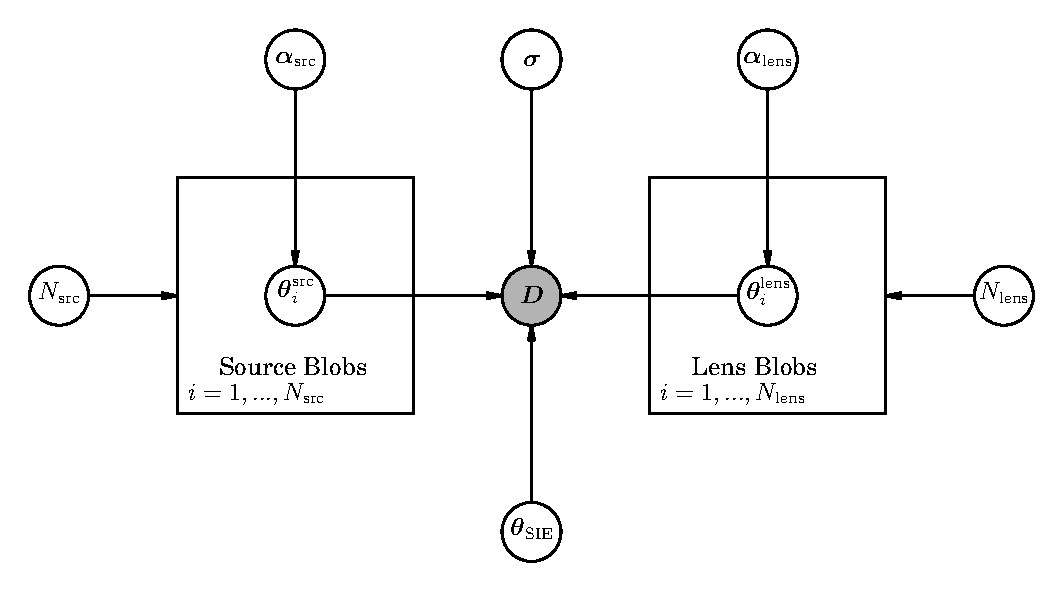
\includegraphics{pgm.pdf}
\caption{A probabilistic graphical model (PGM) of the dependence structure
of the prior information, produced using DAFT ({\tt www.daft-pgm.org}).
The prior for the source and lens blob parameters are specified conditional
on hyperparameters. The purpose of this is to induce dependence in the prior
distribution for the blob parameters, implying (for example) that the mass of
one blob is slightly informative about the mass of another, and that the
locations might be clustered around a certain typical location.
\label{fig:pgm}}
\end{figure*}

\subsection{Conditional prior for the data}
The conditional prior for the data given the parameters
is a product of independent gaussian distributions, one for each pixel.
The mean of the gaussian is given by the ``mock'' noise-free image we would
expect based on the parameters. The standard deviation of the gaussian is
a combination of three terms; the first (denoted $s_{ij}$) is a ``noise map''
which is loaded from a file, the second is an unknown constant $\sigma_0$
which applies to the whole image, and the third is proportional to the
square root of the mock image, with proportionality constant $\sigma_1$.

This is usually called the ``sampling distribution'', or sometimes just the
``likelihood''. However, sampling distribution is misleading since no
physical frequency distribution exists which is being sampled from. The term
likelihood is also usually used to refer to the scalar function of the parameters
obtained when the data are known. For a discussion of the view that this
object is really a prior distribution, see \citet[][pp. 33--35]{caticha}.

\section{Computation}
Computing the posterior distribution over the parameters of such a model
requires that we can implement Markov Chain Monte Carlo (MCMC) over the space
of possible sources and lenses.

To compute the posterior distribution for the parameters
(of which there are 24--464, depending on the values of $N_{\rm src}$ and
$N_{\rm lens}$), we use Diffusive Nested Sampling \citep{dnest}, a form
of Nested Sampling \citep{skilling} that uses the Metropolis algorithm
to move around the parameter space.

The proposal distributions for the blob parameters (both source and lens) are
handled by the {\tt RJObject} library \citep{rjobject}. This includes
birth and death proposals that increase or decrease either $N_{\rm src}$,
or $N_{\rm lens}$, as well as proposals that move the blobs (in their parameter
space) while keeping the number of blobs fixed. {\tt RJObject} also
facilitates proposals that change the hyperparameters (either for the lens
or the source) while keeping the actual blobs in place, as well as proposals
that change the hyperparameters and shift all of the relevant blobs in
so they are appropriate for the new values of the hyperparameters.

Evaluating likelihood function requires that we compute a ``mock'' image from
the current setting of the parameters. This mock image is calculated using
standard ray-tracing methods with a uniform grid of $n \times n$ rays
fired per image pixel. However, certain kinds of proposals do not affect the
image in any way, such as those that change the noise parameters.

\section{Simulated Data}
To demonstrate the method, we generated a simulated dataset with a single
substructure. The image is shown in Figure~\ref{fig:simulated_image}, and
consists of 100 $\times$ 100 pixels. The PSF was compact and was
defined on a 5 $\times$ 5 grid. The data was created by firing only one ray
per pixel, and the inference was also carried out under the same level of
approximation. Since the model assumptions are all correct for this image, the
demonstration here is purely to illustrate the computational tractability of
the problem, and the kind of outputs the method can produce.

\begin{figure}
\begin{center}
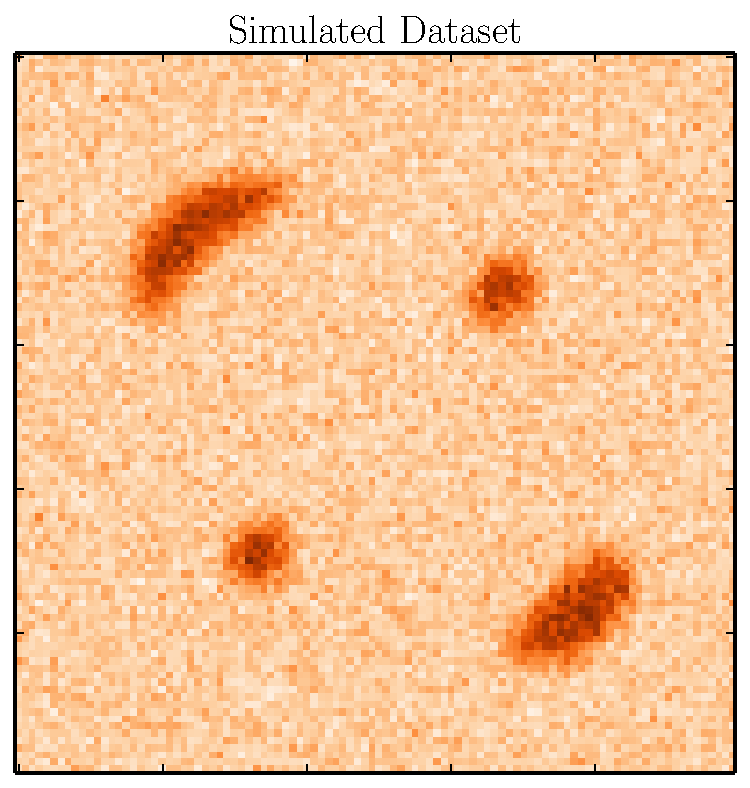
\includegraphics[scale=0.5]{simulated_image.pdf}
\caption{A simulated image of a simple ``galaxy'' lensed by an SIE+$\gamma$
lens plus a single dark substructure. The image was blurred by a PSF and had
some noise added.\label{fig:simulated_image}}
\end{center}
\end{figure}

We executed the code to generate 5,000 samples from the ``mixture of
constrained priors'' distribution of DNest. Our thinning factor was $10^5$,
so $5 \times 10^8$ MCMC iterations were actually performed, taking approximately
48 hours on a PC purchased new in 2012. After resampling these samples to
reflect the posterior distribution, we were left with 537
(equally weighted) posterior samples.

The posterior distributions for complex models, such as the mixture models used here, are often challenging and unintuitive to summarise. One effective way
to visualise the uncertainty in the inferences is to play a movie where each
frame is a sample from the posterior distribution. The degree to which the
frames differ from each other conveys the uncertainty remaining after taking
the data into account.

The {\it empirical measure} of the substructure positions is a function that
takes the substructure positions $(x_i^{\rm lens}, y_i^{\rm lens})$ and
produces a ``density function'' over two dimensions, composed of delta
functions at the positions themselves:
\begin{eqnarray}
\left\{
(x_i^{\rm lens}, y_i^{\rm lens})
\right\}_{i=1}^{N_{\rm lens}}
\Longrightarrow
\sum_{i=1}^{N_{\rm lens}}
\delta^2\left(x - x_i^{\rm lens}, y - y_i^{\rm lens}\right).
\end{eqnarray}

Intuitively, the empirical measure is a mathematical object that is like
an ``infinite resolution histogram'', in this case a two dimensional histogram,
of the substructure positions.
Being a function of the actual substructure positions, the empirical measure
is not available to us since we do not know those positions with certainty.
However, we have samples from the posterior distribution for those positions,
and can use these (trivially) to create samples from the posterior distribution
for the empirical measure. We can also summarise this posterior, for example,
by taking its expected value.

The posterior expected value of the empirical measure is:
\begin{eqnarray}
\int p(\boldsymbol{\theta} | \boldsymbol{D})
\sum_{i=1}^{N_{\rm lens}}
\delta^2\left(x - x_i^{\rm lens}, y_i^{\rm lens} - y_i^{\rm lens}\right)
\, d\boldsymbol{\theta}
\end{eqnarray}
where $\boldsymbol{\theta}$ denotes all parameters and hyperparameters
(including the $N$s) and ``$\int \,d\boldsymbol{\theta}$'' is an integral and summation over the entire parameter space.

Since we can approximate posterior expectations using Monte Carlo, we can
obtain the expected value of the empirical measure using:
\begin{eqnarray}
\frac{1}{n}
\sum_{k=1}^n
\sum_{i=1}^{N_{\rm lens}}
\delta^2\left(x - x_i^{\rm lens}, y_i^{\rm lens} - y_i^{\rm lens}\right)
\end{eqnarray}
where $n$ is the number of posterior samples. The resulting function is
an ``image'' with a point mass wherever a substructure occurred. For
visualisation purposes the image can be blurred, or calculated at a lower
resolution by replacing the Dirac-delta function with a discrete version
which returns a nonzero constant
if a substructure appears in a pixel or zero otherwise.

The masses of the smooth and substructure components of the lens are usually
of interest. Since the total mass of an SIE lens is infinite, the question
needs to be redefined, so we ask about the mass within some aperture of finite
area. For an SIE, the mass (in dimensionless units) within the critical
ellipse is simply $b^2$. However, the blobs have finite total masses
$\{M_i\}$. To obtain the posterior distribution for the lens masses, one must
be clear about exactly which mass they are talking about, and many definitions
are possible, although some might be more meaningful or well constrained than
others.

In the present paper we do not address the question of exactly which quantities
related to the
density profile of the lens are most scientifically interesting. Nevertheless,
we can verify that the results of the inference do behave in understandable
ways. For example, in Figure~\ref{fig:simdata_masses},
we plot the joint posterior distribution
for the SIE mass within its critical ellipse and the total substructure mass
over the entire domain. As one would expect, there is a strong dependence
between these two quantities in the posterior distribution, as mass in the
SIE can be traded off with mass in substructures to some extent, while
the model remains (loosely speaking) ``consistent with the data''.
\begin{figure}
\begin{center}
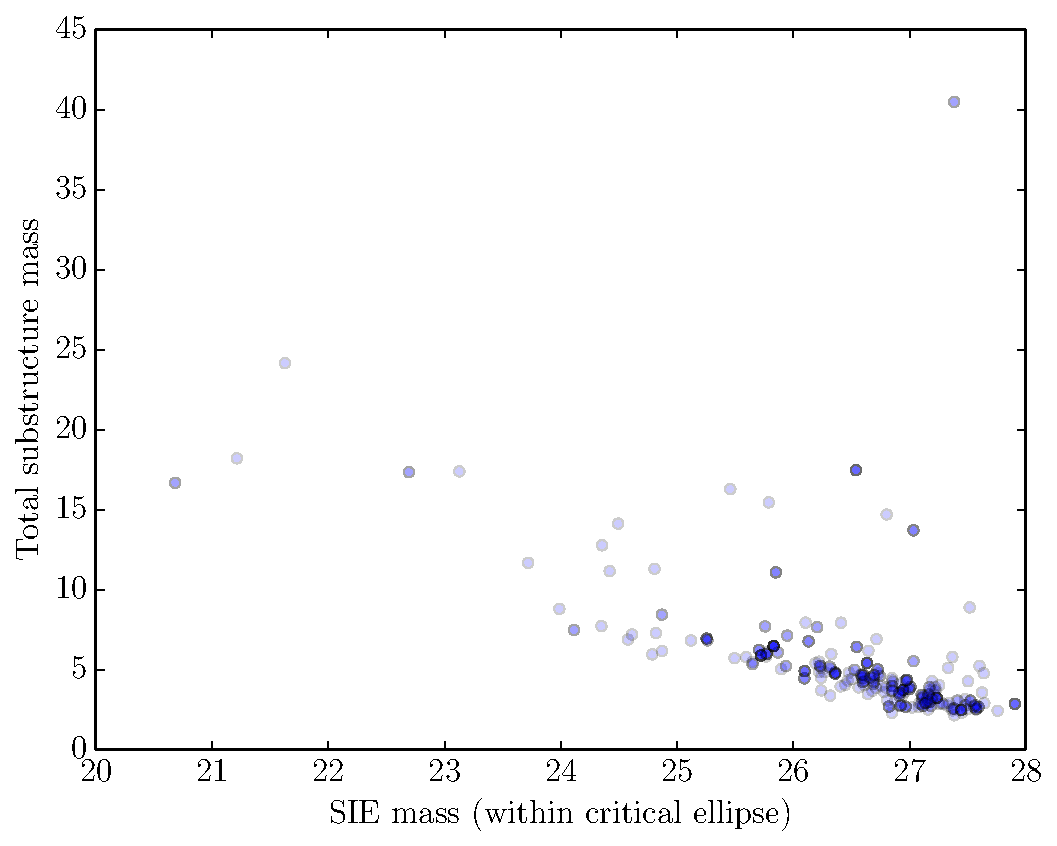
\includegraphics[scale=0.4]{simdata_masses.pdf}
\caption{The joint posterior distribution for the SIE mass (integrated within
its critical ellipse, which is not the critical curve of the lens overall),
and the total mass in substructures.\label{fig:simdata_masses}}
\end{center}
\end{figure}

The posterior distribution for $N_{\rm lens}$ is also clearly of interest, and
is displayed in Figure~\ref{fig:N_lens}. The prior for this parameter was
uniform from 0 to 10 (inclusive), and the possibility $N=0$ has been
(loosely speaking) ``ruled out'' by the image data. The true solution ($N=1$)
has the highest probability. However, the possibilities with $N > 1$ are
still fairly plausible, since it's possible that a very small substructure
exists, and it's also possible that two substructures near each other could
mimic the effect of one. The degree to which these possibilities are plausible
is related to the choice of prior for the blob amplitudes and positions.

\begin{figure}
\begin{center}
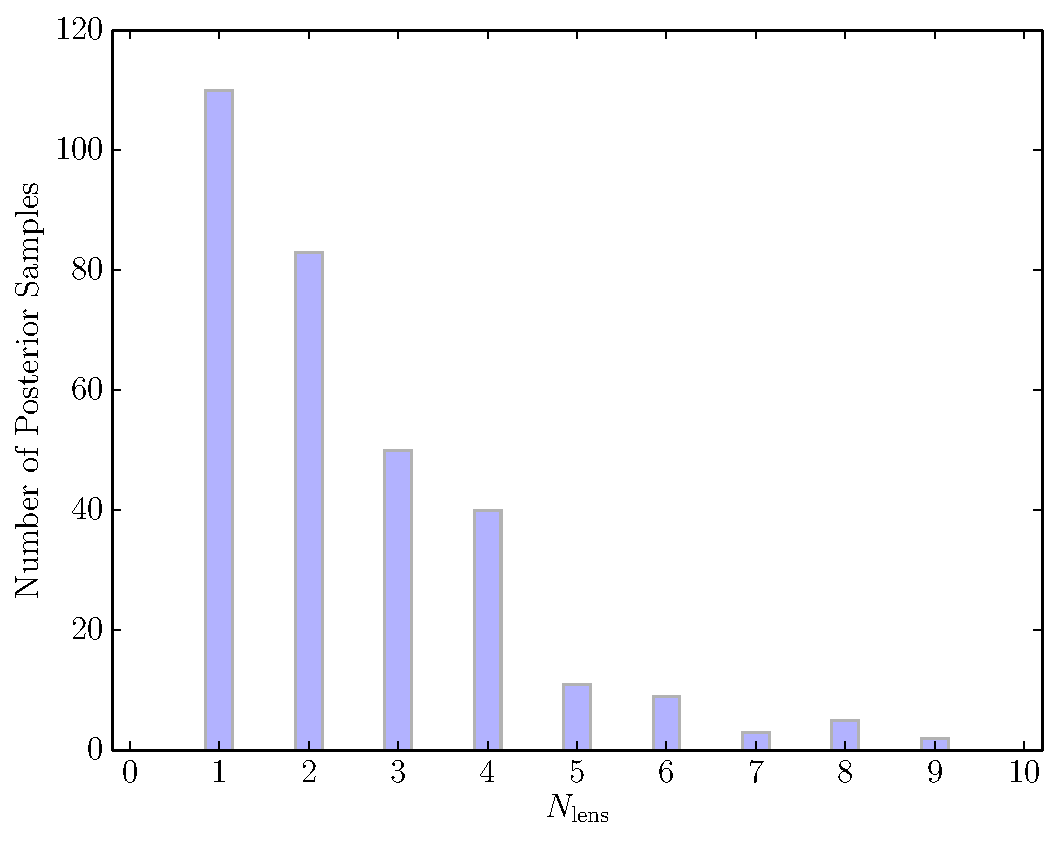
\includegraphics[scale=0.4]{N_lens.pdf}
\caption{The marginal posterior distribution for $N_{\rm lens}$, the
number of substructures in the lens. The prior was uniform and the true
value used to generate the data was 1. However, the data is only informative
enough to suppress the probability of values above 1 slightly, since it
is possible (given this data) that low mass substructures might exist somewhere,
or that what we think is one substructure might actually be two close together,
and other such possibilities.
\label{fig:N_lens}}
\end{center}
\end{figure}

The estimated marginal likelihood of our model
(averaged over all parameters including $N_{\rm lens}$ and $N_{\rm src}$)
is
$\ln\left[p(\boldsymbol{D} | \boldsymbol{\theta})\right] \approx -14248$, and
the information (Kullback-Leibler divergence from the prior to the posterior)
is $\mathcal{H} \approx 99$ nats. The information represents the degree of
compression of the posterior distribution with respect to the prior, and can
be interpreted quite literally as how much was learned about the parameters from
the data. It is also straightforward to estimate from Nested Sampling
\citep{skilling}. Its definition is:
\begin{eqnarray}
\mathcal{H} = \int p(\boldsymbol{\theta} | \boldsymbol{D})
\ln\left[\frac{p(\boldsymbol{\theta} | \boldsymbol{D})}{p(\boldsymbol{\theta})}\right]
\, d\boldsymbol{\theta}
\end{eqnarray}
and we can build intuition about its meaning based on some simple examples. One
such example is a uniform prior over a volume $V_0$ and a posterior which is
uniform over a smaller volume $V_1$ contained within $V_0$. In this case
$\mathcal{H} = \ln(V_0/V_1)$ nats. Therefore, a value of $\mathcal{H}=100$ nats
implies the posterior distribution occupies roughly $e^{-100}$ of the prior
volume.

\begin{figure}
\begin{center}
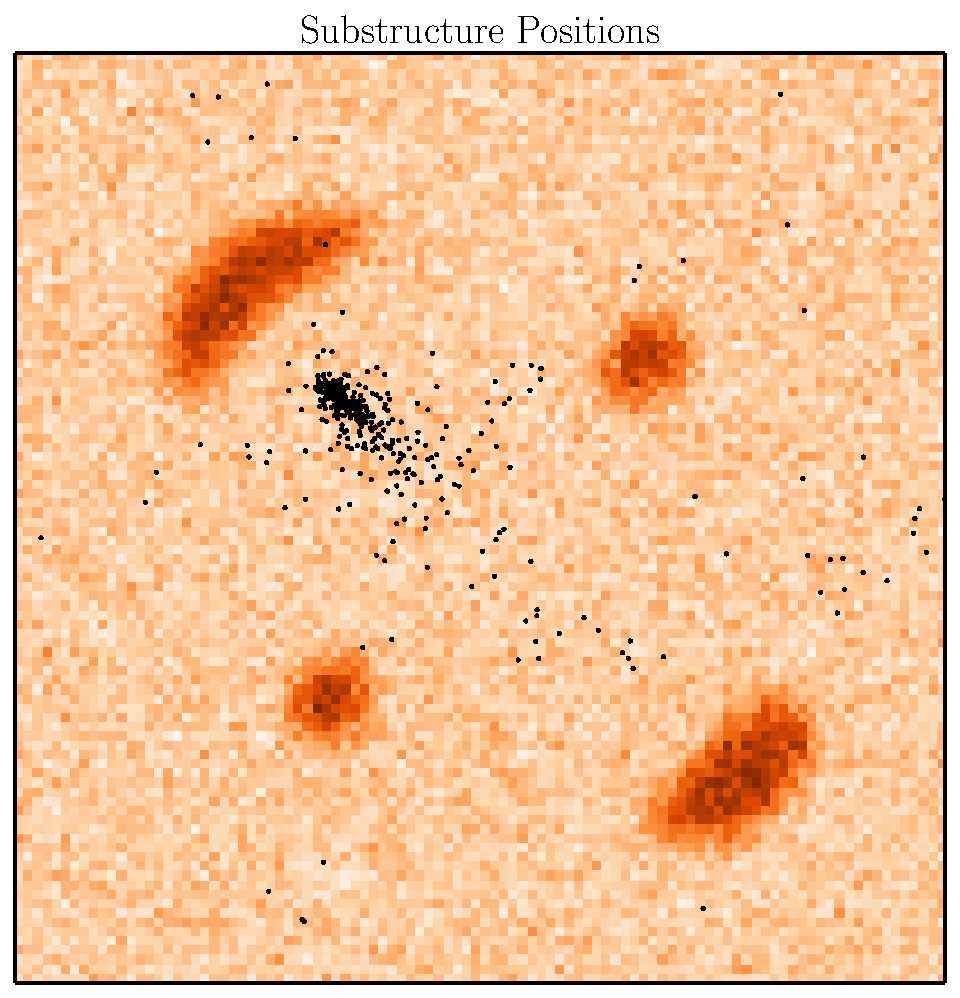
\includegraphics[scale=0.4]{substructures.pdf}
\caption{The simulated data, with substructure positions overlaid (a
Monte Carlo approximation to the posterior expectation of the empirical
measure).
\label{fig:substructures}}
\end{center}
\end{figure}



\section{The Cosmic Horseshoe}
As a further demonstration the method, we apply it to the X-band data
from the Isaac Newton Telescope (INT). This image of the Cosmic Horseshoe
\citep{}, which is shown in Figure~\ref{fig:horseshoe_image}. For this system,
more data is available (Y and Z band data, as well as more recent
Hubble Space Telescope (HST) imaging). Unfortunately our current implementation
doesn't allow for multi-band data (unlike \citet{2011MNRAS.412.2521B}), and
is quite slow when running on the larger HST image. Therefore this section
should be considered a further demonstration of the technique, and not a
thorough study of this system.

We generated 5,000 samples from the DNest target distribution and thinned
by a factor of $10^5$, so $5 \times 10^8$ MCMC iterations were actually
performed, taking approximately 40 hours. The first 1/3 of the run was
excluded as burn-in. After resampling, this resulted in 632
equally weighted posterior samples. Although this image is smaller than the
simulated data ($46 \times 46$ pixels), we fired $2 \times 2$ rays per pixel
for greater accuracy.


%The field of view of the image is $15.3180" \times 15.3180"$, and the size is $46 \times 46$ pixels, therefore one pixel is equivalent to $0.33"$. \\
%The method discussed  in the previous section is applied to two models, the first model consist of a flexible source and a Singular Isothermal Elliptical(SIE) model for the lens. This model is has been used often  \cite{Dye2008}, \cite{schneider_falcoa_Ehlers_1994},      . 
%The second model has in addition to the flexible source and SIE, also possible satellites. \\
%The amount of added satellites is automatically determined by the program. If models the addition of an satellite galaxies gives a higher probability it will be preferred over then model without satellite galaxies.  \\
%In both models the SIE is specified by the usual parameters: the location of the SIE ($x_c$,$y_c$), b, axis ratio $f$\footnote{in the code denoted with $q$},  the core radius$\zeta$, $\theta$, shear $\gamma$, and $\theta_{\gamma}$ \cite{kormann_schneider_1994}.\\

\begin{figure}
\begin{center}
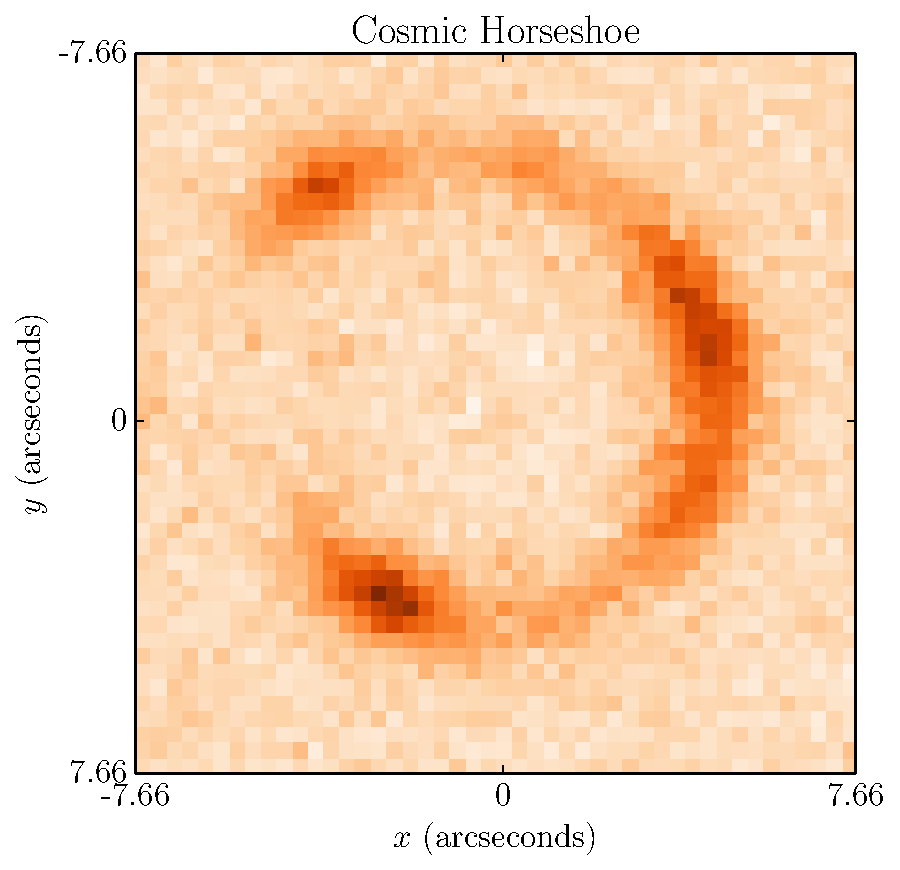
\includegraphics[scale=0.5]{horseshoe_image.pdf}
\caption{\label{fig:horseshoe_image}}
\end{center}
\end{figure}


\begin{figure}
\begin{center}
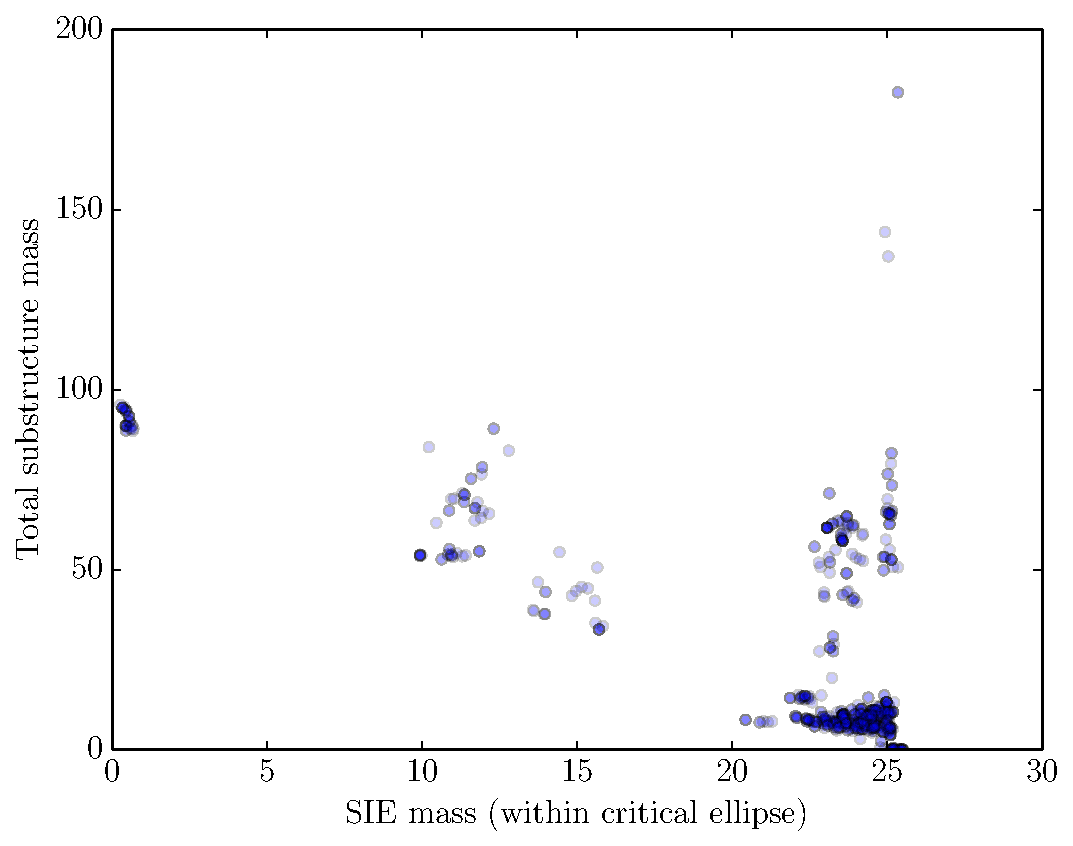
\includegraphics[scale=0.4]{masses2.pdf}
\caption{The joint posterior distribution for the SIE mass (integrated within
its critical ellipse, which is not the critical curve of the lens overall),
and the total mass in substructures.\label{fig:simdata_masses}}
\end{center}
\end{figure}

\begin{figure}
\begin{center}
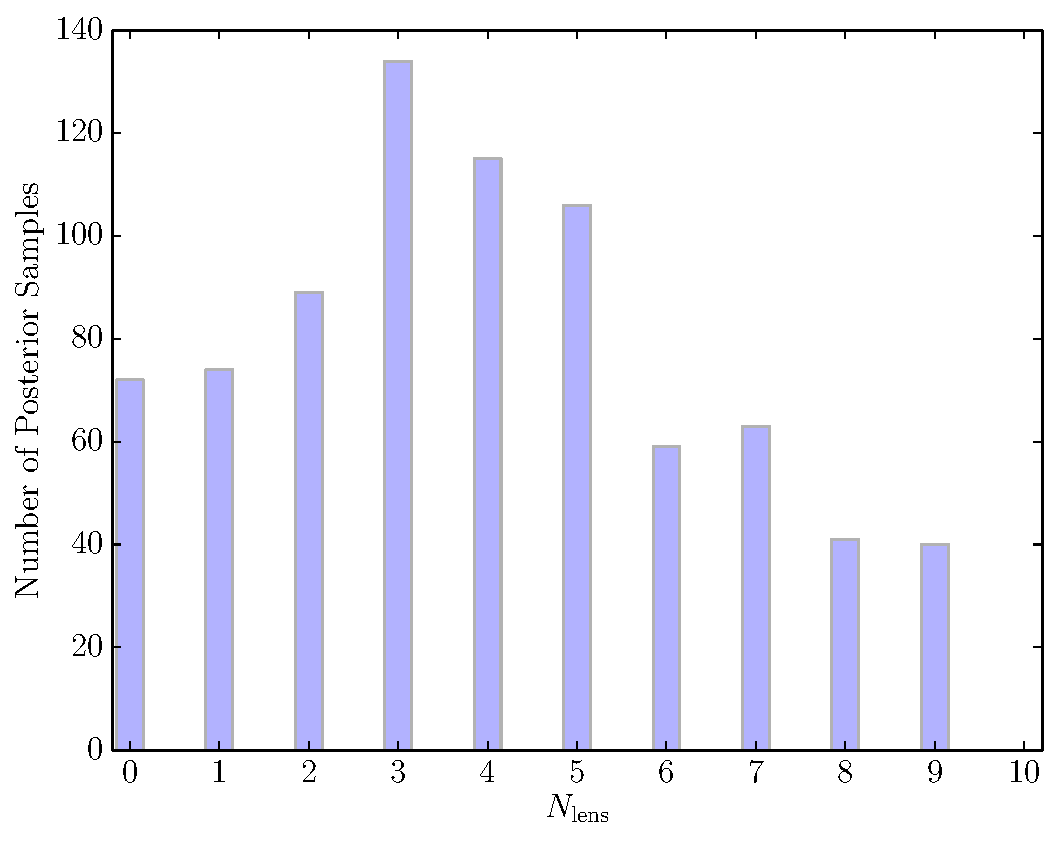
\includegraphics[scale=0.4]{N_lens2.pdf}
\caption{\label{fig:N_lens2}}
\end{center}
\end{figure}

\begin{figure}
\begin{center}
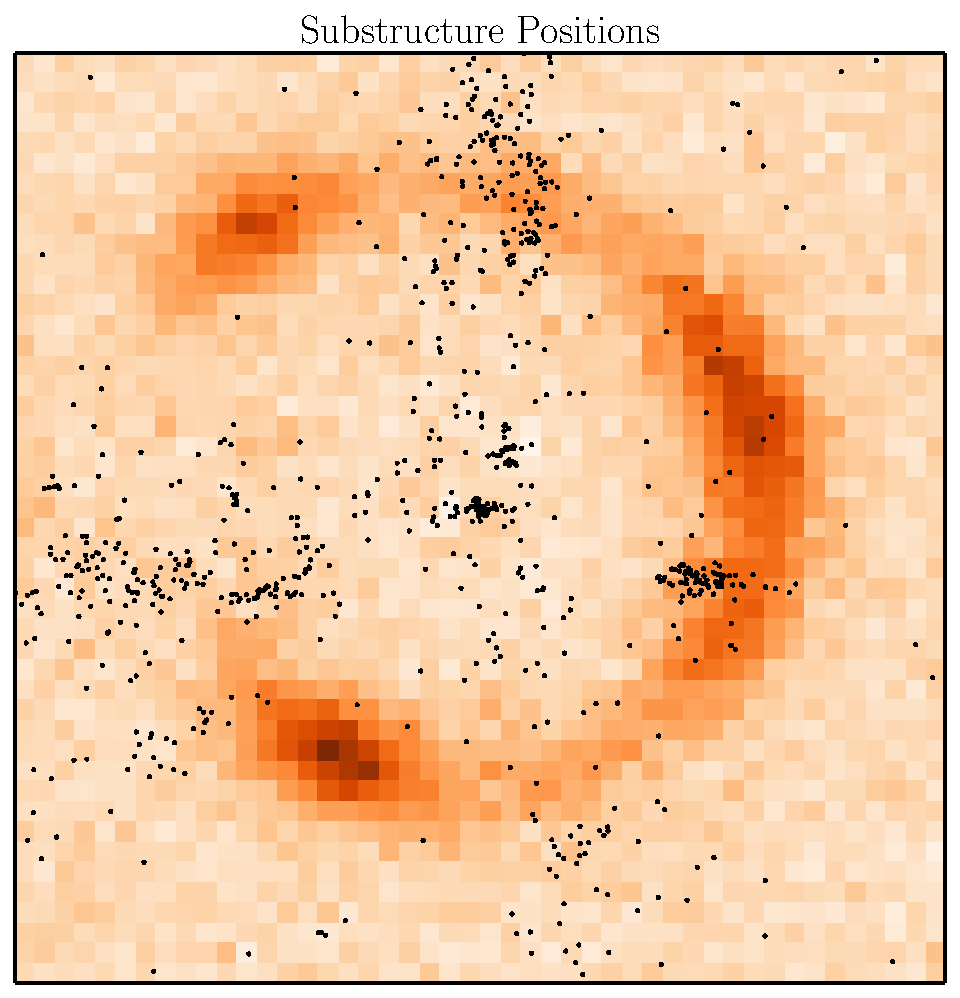
\includegraphics[scale=0.4]{substructures2.pdf}
\caption{\label{fig:substructures2}}
\end{center}
\end{figure}

The estimated marginal likelihood of our model
is
$\ln\left[p(\boldsymbol{D} | \boldsymbol{\theta})\right] \approx -6967$, and
the information (Kullback-Leibler divergence from the prior to the posterior)
is $\mathcal{H} \approx 129$ nats.

\subsection{Reproducibility of the results}
The ``effective sample size'' returned by DNest, which we have described as the
number of posterior samples, takes into account the fact DNest's target
distribution is not the posterior. However, it does not take autocorrelation
into account, and thus can present an optimistic picture of the accuracy of
any Monte Carlo approximations to posterior quantities. Most standard diagnostic
techniques used in MCMC can be applied here. The simplest of these is a
check of reproducibility. If different runs yield substantially different
results, the MCMC output should be treated with caution.

% \begin{figure*}
%% \hspace{20pt}
%\begin{subfigure}{.45\textwidth}
%  \centering
%  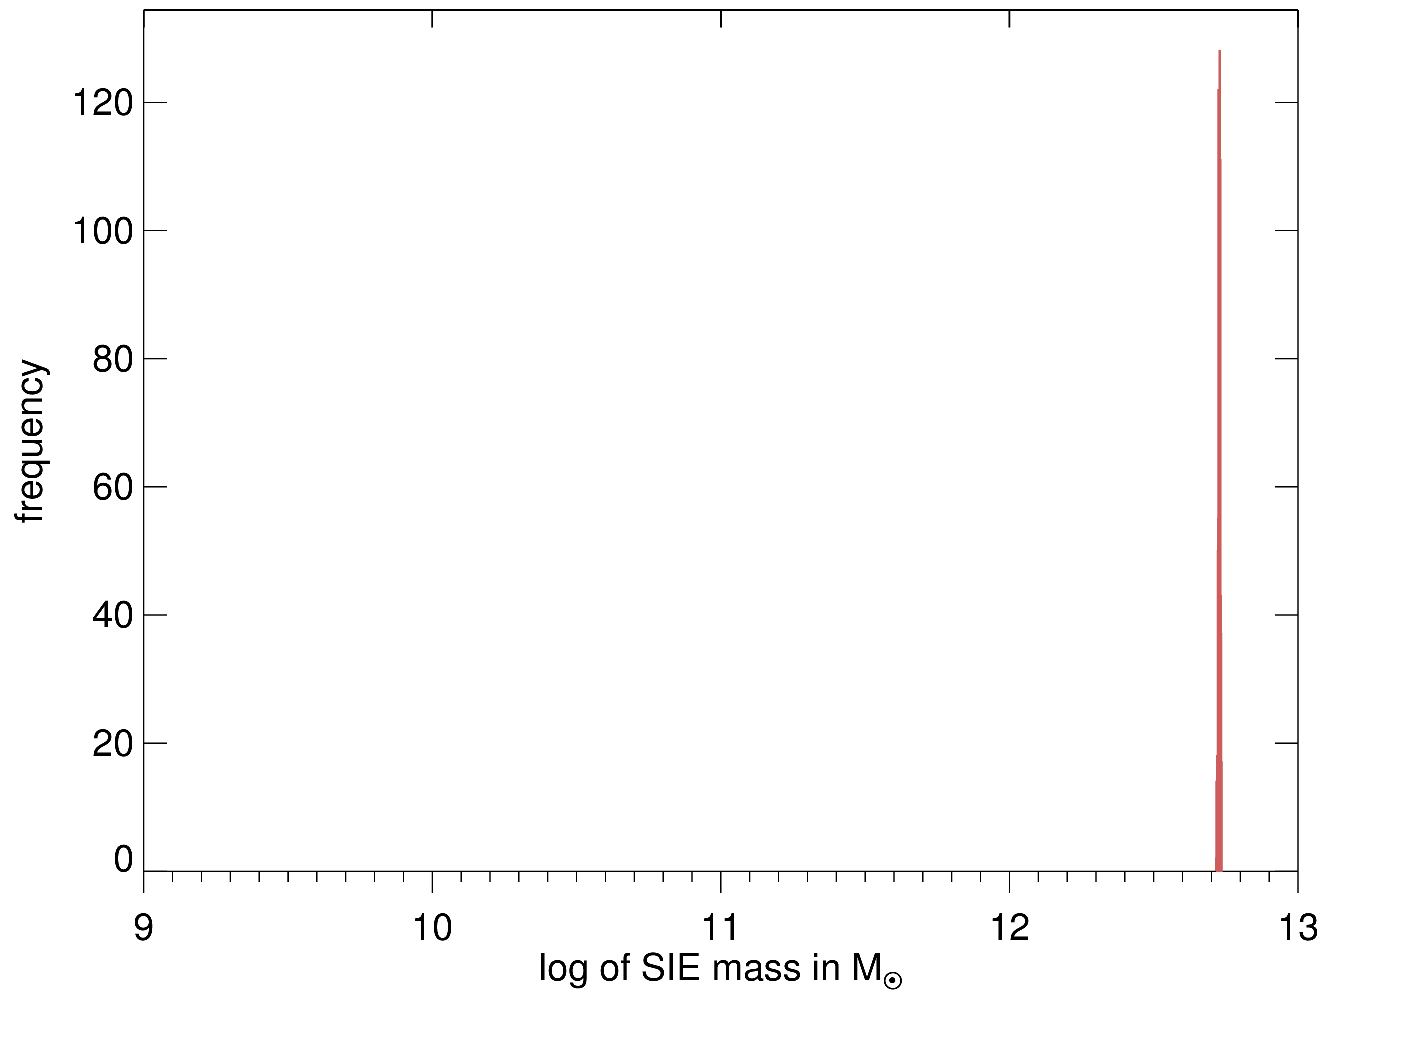
\includegraphics[width=0.75\linewidth,angle=90]{log_mass_SIE_no_blobs.eps}
%\parbox{0.8\linewidth}{\caption{The log of the SIE mass within the critical curve  for model A.  \label{fig:sub1} }}
%\end{subfigure}%
%\begin{subfigure}{.45\textwidth}
%  \centering
%  
\includegraphics[width=0.75\linewidth,angle=90]{log_mass_SIE.eps}
%   \parbox{0.8\linewidth}{\caption{The log of the SIE mass within the critical curve for model B.   \label{fig:sub2}}}
%\end{subfigure}
%   \end{figure*}

%After choosing the prior probabilities one has to initialized the Dnest-code, which mean incorporating the problem specific information for
% example dimensions of the images in pixels, image size in arc-seconds, information on the PSF etc in the metadata file. 
% Besides these problem specific parameters, there are also several other parameters concerning the performance of code which need to be
%  edited in the OPTION file. After these initialization, we ran a test run to explore the amount of necessary levels, and length of the run.
% A sufficiently amount of levels correlates with good degree of mixing, and the length of the run is associated with the larger sample
%  size. After one test run, the amount levels was adapted to 120, and the amount iterations was change to 5000 iterations, for model A this resulted in the effective sample size of 940, and for model B this resulted in the effective sample size of 757.  The difference between the effective sample size is not unexpected, since the probability space which can be explored by applying model B much larger.  \\
%Throughout the paper the standard cosmology was used for the analysis:  $H_0=70 \rm{km~s^{-1} ~pc^{-1}}$,  $\Omega_m = 0.3$,and  $\Omega_\Lambda= 0.7$. 
%The first test would to compare the SIE-mass of the models with the mass obtained in previous  work \cite{Belokurov2007} \cite{Dye2008}.
%Using model A the median  calculated SIE mass within the critical curve in solar masses is  $(5.34 \pm 0.046) \cdot 10^{12} M_\odot$, % (using median + STDDEV)
%which is comparable with previous work which gave the enclosed (cylindriacal) mass $(5.4 \pm 0.09) \cdot 10^{12} M_\odot$ \cite{Belokurov2007} and  mass within the Einstein-ring $(5.02 \pm 0.09) \cdot 10^{12} M_\odot$ \cite{Dye2008}. Figure \ref{fig:sub1} displays the histogram of the enclosed mass within an Einstein ring of $5"$, it displays a very well confined probability distribution of the mass. \\ 
%Using model B the median calculated SIE mass within the critical curve in solar masses is  $(5.34 \pm 0.046) \cdot 10^{12} M_\odot$, % (using median + STDDEV)
%which is slightly smaller compared to the masses obtained with model A and the masses from previous work mentioned above. Which is also not unexpected, because models where the SIE-mass is smaller can compensate by adding a satellite near by. Therefore the distribution is much wider as one can see in figure \ref{fig:sub2}. The median of the SIE-mass in model B is $(4.79 \pm 1.66) \cdot 10^{12} M_\odot$, which leaves a large numerical uncertainty. However by comparison of the two histograms in figure \ref{fig:1} it is apparent that the distribution has a strong feature at the location. \\
% 
%\begin{figure}[!h]
%\hspace{5pt}
%\begin{subfigure}{.45\textwidth}
%  \centering
%  
\includegraphics[width=0.7\linewidth,angle=90]{log_total_mass_blob.eps}
%\parbox{0.8\linewidth}{\caption{The log of the total mass of the satellites for model B.   \label{fig:sub3}}}
%\end{subfigure}%
%\hspace{-15pt}
%\begin{subfigure}{.45\textwidth}
%  \centering
%  \vspace{6pt}
%  
\includegraphics[width=0.7\linewidth,angle=90]{log_total_mass_blobs_within_ring.eps}
%\parbox{0.8\linewidth}{\caption{The log of the total mass of the satellites within the fixed Einstein-radius for model B.  \label{fig:sub4} }}
%\end{subfigure}
%   \end{figure}
%\vspace{-15pt}
%\noindent Another interesting aspect is the mass of the satellites. Figure \ref{fig:sub3} displays a histogram of the logarithm of the total mass of the satellites per sample. Figure \ref{fig:sub4} displays histogram of the logarithm of the total mass of the satellites within a radius of $ 5"$ from the centre of images per sample. Comparing these two images reveals that large part the massive satellites lie outside the Einstein ring. The satellites at a larger distance can only influence the images if they are more massive. Figure \ref{fig:sub5} display a histogram of the log of the total mass of the SIE and the satellites within the Einstein radius, which clearly looks very similar to \ref{fig:sub1}. 
%Figure \ref{fig:sub6} display a plot of the total mass of the SIE versus mass of the satellites within the Einstein radius whichs  negative correlation of approximately 
%\begin{equation}
% \sum M_{satellites} = 5\cdot10^{12} - M_{SIE}
% \end{equation}

%The main conclusion of the analysis of the datasets of model A and model B, would be that the application of the DNest code with a free amount of satellite galaxies return a well matching model which is very similar to to the model without any satellites, this proves 
%even though the code has the freedom the explore and create all sort of models, it confirms that the already known distribution is very probable. This shows how well the code works, and beside that it is also good indication that the well established SIE model for this system doesn't need additional satellites to explain the system. 
% 
%\begin{figure}
%\hspace{10pt}
%\begin{subfigure}{.5\textwidth}
%\vspace{-12pt}
%  \centering
%  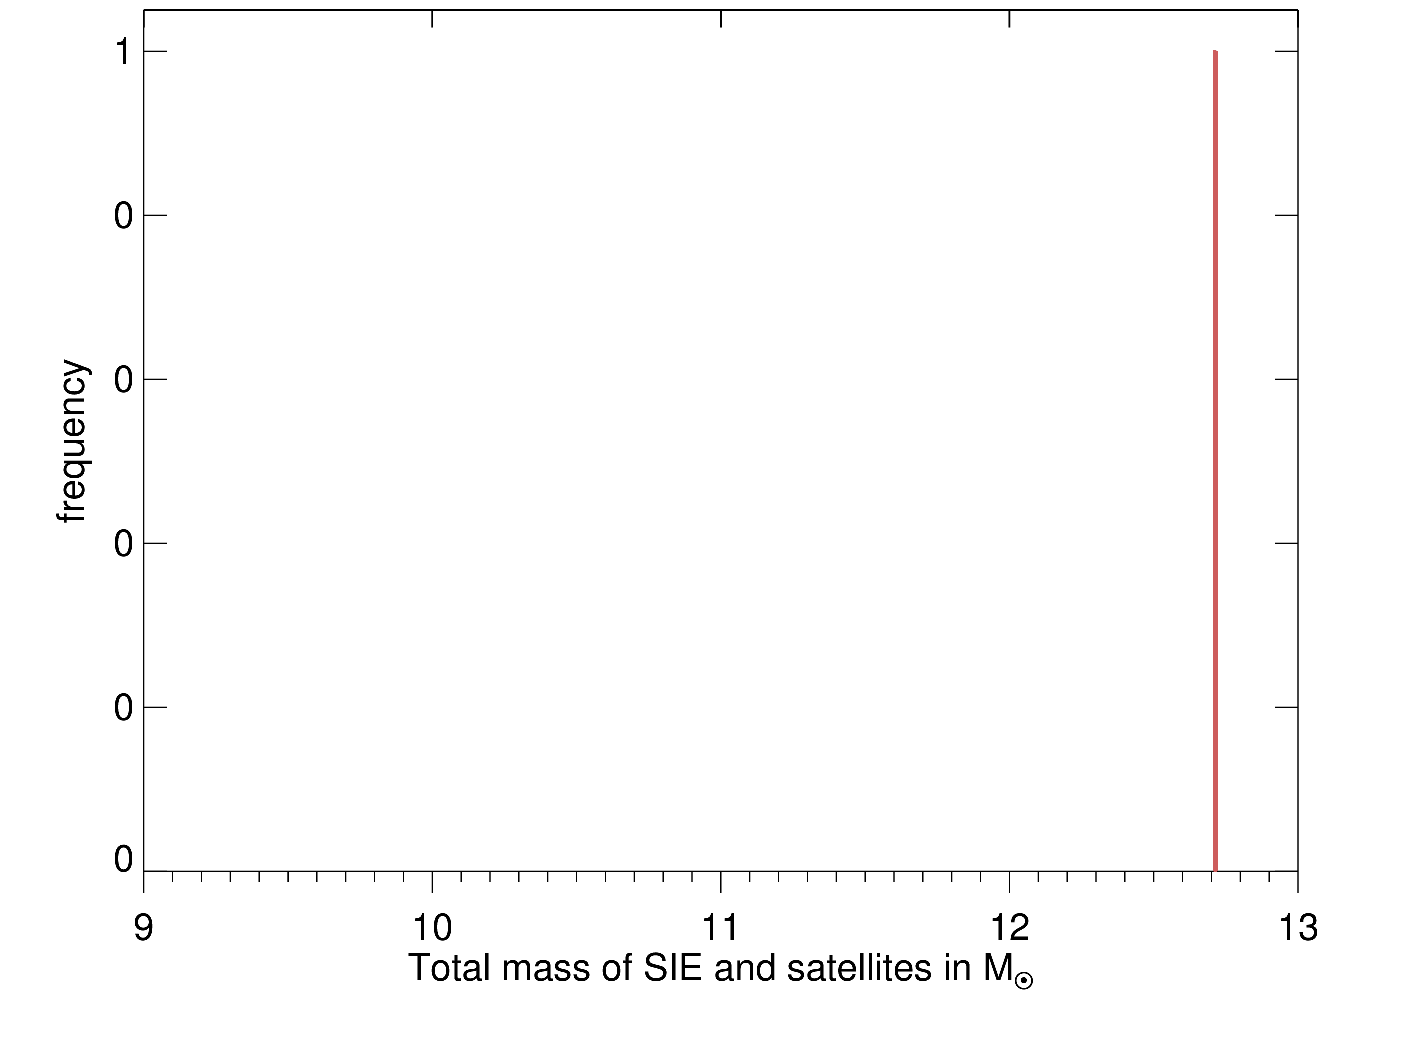
\includegraphics[width=0.75\linewidth,angle=90]{mass_SIE_plus_blob_mass.eps}
%\parbox{0.8\linewidth}{\caption{The log of add mass of the satellites and SIE within the fixed Einstein-radius for model B.   \label{fig:sub5}}}
%\end{subfigure}
%\begin{subfigure}{.5\textwidth}
%  \centering
%  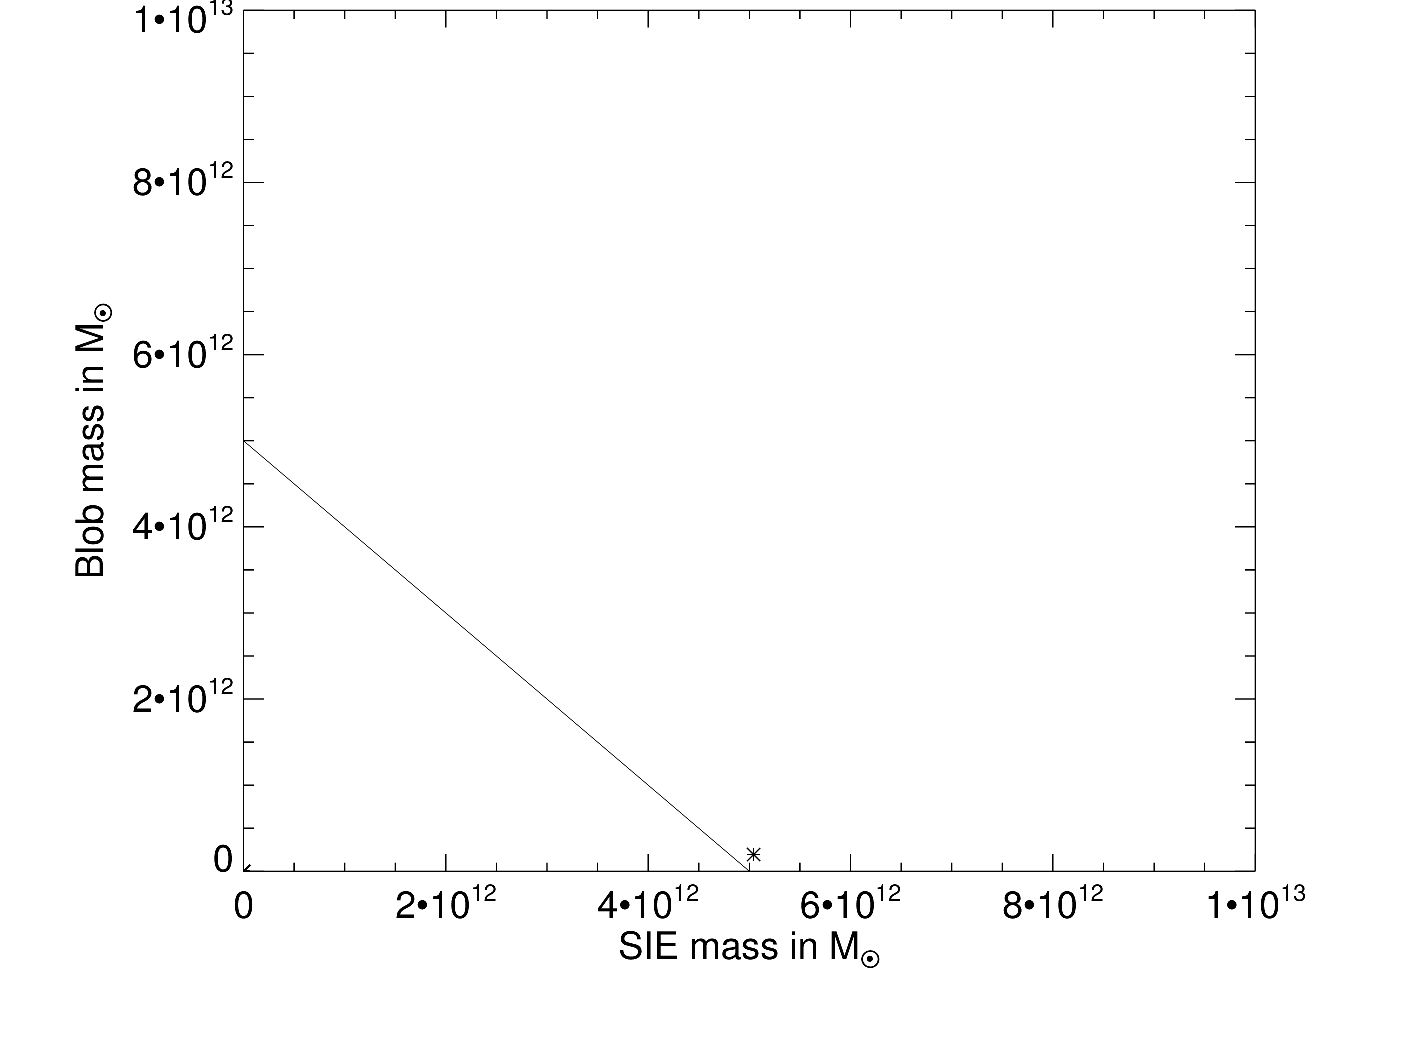
\includegraphics[width=0.75\linewidth,angle=90]{joint.eps}
%\parbox{0.8\linewidth}{\caption{Plot of the log of the total mass of the satellites within the fixed Einstein-radius versus the 
%log of the SIE mass within the Einstein radius for model B.  \label{fig:sub6} }}
%\end{subfigure}

%   \end{figure}

%  
%  

%\section{ER 0047-2808}
%We demonstrate the method on the HST images of ER 0047-2808.

\section*{Acknowledgements}
It is a pleasure to thank Phil Marshall (Stanford) and Tommaso Treu (UCLA)
for valuable discussion.

This work was funded by a Marsden Fast Start grant from the Royal Society of
New Zealand.


\begin{thebibliography}{99}
\bibitem[\protect\citeauthoryear{Birrer, Amara, 
\& Refregier}{2015}]{2015arXiv150407629B} Birrer S., Amara A., Refregier A., 2015, arXiv, arXiv:1504.07629

\bibitem[\protect\citeauthoryear{Brewer 
\& Lewis}{2006}]{2006ApJ...637..608B} Brewer B.~J., Lewis G.~F., 2006, ApJ, 637, 608

\bibitem[\protect\citeauthoryear{Brewer, P{\'a}rtay,
\& Cs{\'a}nyi}{2011}]{dnest} Brewer B.~J., P{\'a}rtay L.~B., Cs{\'a}nyi G., 2011,
Statistics and Computing, 21, 4, 649-656. arXiv:0912.2380

\bibitem[\protect\citeauthoryear{Brewer et al.}{2011}]{2011MNRAS.412.2521B} 
Brewer B.~J., Lewis G.~F., Belokurov V., Irwin M.~J., Bridges T.~J., Evans 
N.~W., 2011, MNRAS, 412, 2521

\bibitem[\protect\citeauthoryear{Brewer}{2014}]{rjobject} Brewer, B. J., 2014,
preprint. ArXiv: 1411.3921

\bibitem[\protect\citeauthoryear{Brewer 
\& Donovan}{2015}]{exoplanet} Brewer B.~J., Donovan C.~P., 2015, MNRAS, 448, 3206 

\bibitem[Caticha(2008)]{caticha} Caticha, A.\ 2008.\ Lectures 
on Probability, Entropy, and Statistical Physics.\ ArXiv e-prints 
arXiv:0808.0012. 

\bibitem[\protect\citeauthoryear{Coles, Read, 
\& Saha}{2014}]{2014MNRAS.445.2181C} Coles J.~P., Read J.~I., Saha P., 2014, MNRAS, 445, 2181

\bibitem[\protect\citeauthoryear{Fadely 
\& Keeton}{2012}]{2012MNRAS.419..936F} Fadely R., Keeton C.~R., 2012, MNRAS, 419, 936

\bibitem[\protect\citeauthoryear{Green}{1995}]{rjmcmc}
Green, P.~J., 1995, Reversible Jump Markov Chain Monte Carlo Computation and Bayesian Model Determination, Biometrika 82 (4): 711–732.

\bibitem[\protect\citeauthoryear{Grillo et al.}{2015}]{grillo} 
Grillo C., et al., 2015, ApJ, 800, 38 

\bibitem[\protect\citeauthoryear{Huppenkothen et 
al.}{2015}]{magnetron} Huppenkothen D., et al., 2015,
accepted for publication in ApJ. arXiv:1501.05251 

\bibitem[\protect\citeauthoryear{Koopmans}{2005}]{koopmans} 
Koopmans L.~V.~E., 2005, MNRAS, 363, 1136

\bibitem[\protect\citeauthoryear{Kormann, Schneider, 
\& Bartelmann}{1994}]{1994A&A...284..285K} Kormann R., Schneider P., Bartelmann M., 1994, A\&A, 284, 285

\bibitem[\protect\citeauthoryear{O'Hagan and Forster}{2004}]{ohagan}
O'Hagan, A., Forster,~J., 2004, Bayesian inference. London: Arnold.

\bibitem[\protect\citeauthoryear{Sivia \& Skilling}{2006}]{sivia} Sivia, 
D.~ S., Skilling, J., 2006, Data Analysis: A Bayesian Tutorial, 2nd 
Edition, Oxford University Press

\bibitem[\protect\citeauthoryear{Skilling}{2006}]{skilling} Skilling, 
J., 2006, ``Nested Sampling for General Bayesian Computation'', Bayesian 
Analysis 4, pp. 833-860

\bibitem[\protect\citeauthoryear{Suyu et al.}{2006}]{suyu} 
Suyu S.~H., Marshall P.~J., Hobson M.~P., Blandford R.~D., 2006, MNRAS, 
371, 983

\bibitem[\protect\citeauthoryear{Suyu et al.}{2014}]{2014ApJ...788L..35S} 
Suyu S.~H., et al., 2014, ApJ, 788, L35 

\bibitem[\protect\citeauthoryear{Suyu et al.}{2013}]{2013ApJ...766...70S} 
Suyu S.~H., et al., 2013, ApJ, 766, 70 

\bibitem[\protect\citeauthoryear{Tagore 
\& Jackson}{2015}]{2015arXiv150500198T} Tagore A.~S., Jackson N., 2015, arXiv, arXiv:1505.00198

\bibitem[\protect\citeauthoryear{Treu}{2010}]{treu} Treu T., 2010, ARA\&A, 48, 87 

\bibitem[\protect\citeauthoryear{Vegetti 
\& Koopmans}{2009}]{2009MNRAS.400.1583V} Vegetti S., Koopmans L.~V.~E., 2009, MNRAS, 400, 1583

\bibitem[\protect\citeauthoryear{Vegetti et 
al.}{2012}]{vegetti1} Vegetti S., Lagattuta D.~J., McKean J.~P., 
Auger M.~W., Fassnacht C.~D., Koopmans L.~V.~E., 2012, Natur, 481, 341 

\bibitem[\protect\citeauthoryear{Vegetti, Czoske, 
\& Koopmans}{2010}]{vegetti3} Vegetti S., Czoske O., Koopmans L.~V.~E., 2010, MNRAS, 407, 225

\bibitem[\protect\citeauthoryear{Vegetti et 
al.}{2010}]{vegetti2} Vegetti S., Koopmans L.~V.~E., Bolton A., 
Treu T., Gavazzi R., 2010, MNRAS, 408, 1969 

\bibitem[\protect\citeauthoryear{Vegetti et 
al.}{2014}]{2014MNRAS.442.2017V} Vegetti S., Koopmans L.~V.~E., Auger 
M.~W., Treu T., Bolton A.~S., 2014, MNRAS, 442, 2017 


\bibitem[\protect\citeauthoryear{Warren 
\& Dye}{2003}]{2003ApJ...590..673W} Warren S.~J., Dye S., 2003, ApJ, 590, 673
\end{thebibliography}


\end{document}

